\documentclass[11pt,]{article}
\usepackage[left=1in,top=1in,right=1in,bottom=1in]{geometry}
\newcommand*{\authorfont}{\fontfamily{phv}\selectfont}
\usepackage[]{mathpazo}


  \usepackage[T1]{fontenc}
  \usepackage[utf8]{inputenc}




\usepackage{abstract}
\renewcommand{\abstractname}{}    % clear the title
\renewcommand{\absnamepos}{empty} % originally center

\renewenvironment{abstract}
 {{%
    \setlength{\leftmargin}{0mm}
    \setlength{\rightmargin}{\leftmargin}%
  }%
  \relax}
 {\endlist}

\makeatletter
\def\@maketitle{%
  \newpage
%  \null
%  \vskip 2em%
%  \begin{center}%
  \let \footnote \thanks
    {\fontsize{18}{20}\selectfont\raggedright  \setlength{\parindent}{0pt} \@title \par}%
}
%\fi
\makeatother




\setcounter{secnumdepth}{0}

\usepackage{longtable,booktabs}

\usepackage{graphicx,grffile}
\makeatletter
\def\maxwidth{\ifdim\Gin@nat@width>\linewidth\linewidth\else\Gin@nat@width\fi}
\def\maxheight{\ifdim\Gin@nat@height>\textheight\textheight\else\Gin@nat@height\fi}
\makeatother
% Scale images if necessary, so that they will not overflow the page
% margins by default, and it is still possible to overwrite the defaults
% using explicit options in \includegraphics[width, height, ...]{}
\setkeys{Gin}{width=\maxwidth,height=\maxheight,keepaspectratio}


\title{End-term project: Advanced Statistical Computing 2020  }



\author{\Large Yizhen Dai\vspace{0.05in} \newline\normalsize\emph{s2395479}  }


\date{}

\usepackage{titlesec}

\titleformat*{\section}{\normalsize\bfseries}
\titleformat*{\subsection}{\normalsize\itshape}
\titleformat*{\subsubsection}{\normalsize\itshape}
\titleformat*{\paragraph}{\normalsize\itshape}
\titleformat*{\subparagraph}{\normalsize\itshape}


\usepackage{natbib}
\bibliographystyle{apsr}
\usepackage[strings]{underscore} % protect underscores in most circumstances



\newtheorem{hypothesis}{Hypothesis}
\usepackage{setspace}


% set default figure placement to htbp
\makeatletter
\def\fps@figure{htbp}
\makeatother

\usepackage{hyperref}

% move the hyperref stuff down here, after header-includes, to allow for - \usepackage{hyperref}

\makeatletter
\@ifpackageloaded{hyperref}{}{%
\ifxetex
  \PassOptionsToPackage{hyphens}{url}\usepackage[setpagesize=false, % page size defined by xetex
              unicode=false, % unicode breaks when used with xetex
              xetex]{hyperref}
\else
  \PassOptionsToPackage{hyphens}{url}\usepackage[draft,unicode=true]{hyperref}
\fi
}

\@ifpackageloaded{color}{
    \PassOptionsToPackage{usenames,dvipsnames}{color}
}{%
    \usepackage[usenames,dvipsnames]{color}
}
\makeatother
\hypersetup{breaklinks=true,
            bookmarks=true,
            pdfauthor={Yizhen Dai (s2395479)},
             pdfkeywords = {Advanced Statistical Computating, Final Project, Simulation},  
            pdftitle={End-term project: Advanced Statistical Computing 2020},
            colorlinks=true,
            citecolor=blue,
            urlcolor=blue,
            linkcolor=magenta,
            pdfborder={0 0 0}}
\urlstyle{same}  % don't use monospace font for urls

% Add an option for endnotes. -----


% add tightlist ----------
\providecommand{\tightlist}{%
\setlength{\itemsep}{0pt}\setlength{\parskip}{0pt}}

% add some other packages ----------

% \usepackage{multicol}
% This should regulate where figures float
% See: https://tex.stackexchange.com/questions/2275/keeping-tables-figures-close-to-where-they-are-mentioned
\usepackage[section]{placeins}


\begin{document}
	
% \pagenumbering{arabic}% resets `page` counter to 1 
%
% \maketitle

{% \usefont{T1}{pnc}{m}{n}
\setlength{\parindent}{0pt}
\thispagestyle{plain}
{\fontsize{18}{20}\selectfont\raggedright 
\maketitle  % title \par  

}

{
   \vskip 13.5pt\relax \normalsize\fontsize{11}{12} 
\textbf{\authorfont Yizhen Dai} \hskip 15pt \emph{\small s2395479}   

}

}








\begin{abstract}

    \hbox{\vrule height .2pt width 39.14pc}

    \vskip 8.5pt % \small 

\noindent This report is the result of the efforts for the final exam/project of
Advanced Statistical Computating. The goal of this project is to analyze
the cost and the benefit of a re-insruance policy through simulation.


\vskip 8.5pt \noindent \emph{Keywords}: Advanced Statistical Computating, Final Project, Simulation \par

    \hbox{\vrule height .2pt width 39.14pc}



\end{abstract}


\vskip -8.5pt


 % removetitleabstract

\noindent  

\hypertarget{introduction}{%
\section{Introduction}\label{introduction}}

\hypertarget{the-goal}{%
\subsection{The goal}\label{the-goal}}

This project aims at solving a modeling problem faced by an insurance
company - ANV. Two of ANV business lines,
\href{https://en.wikipedia.org/wiki/Professional_liability_insurance}{Professional
liability insurance} (PLI) and
\href{https://en.wikipedia.org/wiki/Workers\%27_compensation}{Workers'
compensation} (WC), were affected by a huge claim from one client during
the last year. Therefore, ANV comes to a reinsurance company for an
insurance policy. To put the problem in a mathematical format, we define
the following notation:

\begin{itemize}
\item
  \(X_1\): the loss incurred for PLI from ANV clients (in million
  euros);
\item
  \(X_2\): the loss incurred for WC from ANV clients (in million euros);
\item
  \(t\): the threshold set by the reinsurance company (in million
  euros). For some threshold \(t = 100,110,…,200\), if the total loss
  incurred for PLI and WC from a certain client exceeds \(t\), ANV pays
  the claim themselves; Otherwise, the reinsurance company pays the
  claim.
\item
  \(V(t)\): the expected over-threshold claims, which is equal to
  \(E[(X_1+X_2)1(X_1+X_2>t)]\);
\item
  \(P(t)\): the price that reinsurance company asks. \(P(t)\) depends on
  the threshold \(t\) as \(P(t)=40000 * e^{-t/7}\).
\end{itemize}

Our goal is to determine if ANV should buy such policy from the
reinsurance company. Of course, the policy is only reasonable if the
expected over-threshold claim exceeds the price: \(V(t) > P(t)\). The
data available is the loss incurred for PLI and WC for all the clients
of ANV during last year. With limited data available, we use statistical
modeling to approximate \(V(t)\) and therefore determine if
\(V(t) > P(t)\).

\hypertarget{models}{%
\subsection{Models}\label{models}}

\(X_1\) and \(X_2\) are positively correlated. The correlation between
\(X_1\) and \(X_2\) is 0.528. The linear regression line (in red) and
the \emph{LOWESS} smoother line (in blue) is shown below in Figure 1.

\begin{figure}
\centering
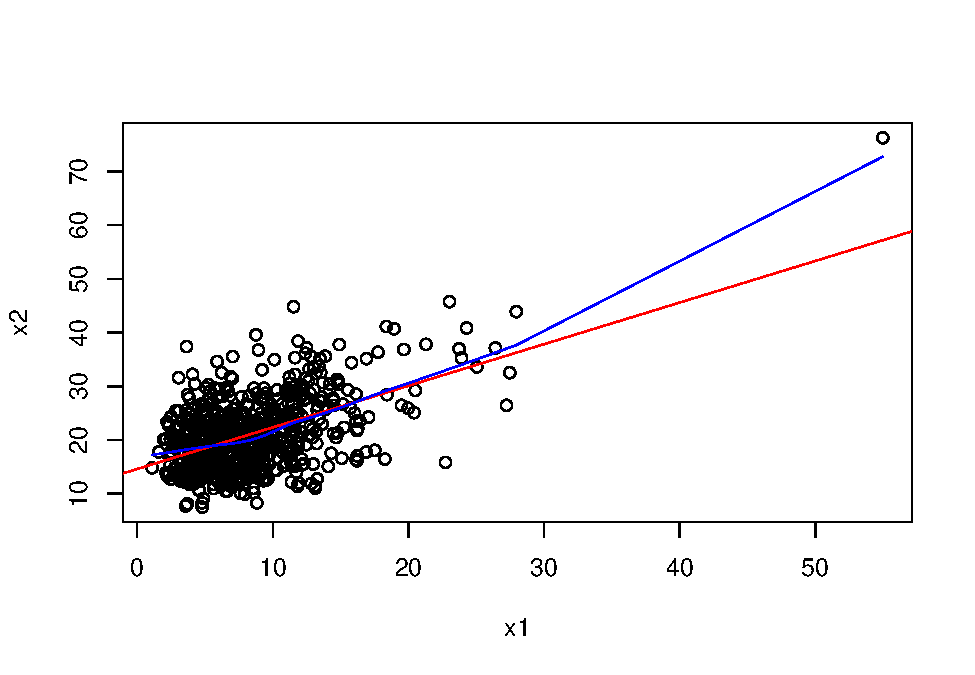
\includegraphics{figs/unnamed-chunk-2.pdf}
\caption{The relationship between X1 and X2}
\end{figure}

In order to reflect the dependence in the data, we cannot simulate
\(X_1\) and \(X_2\) separately. We use a Copula model to model the joint
density \(f_{X_{1}, X_{2}}\).

\[
f_{X_{1}, X_{2}}\left(x_{1}, x_{2}\right)=f_{X_{1}}\left(x_{1}\right) f_{X_{2}}\left(x_{2}\right) c\left(u_1,u_2\right)
\]

where
\(u_1 = F_{X_{1}}\left(x_{1}\right),u2= F_{X_{2}}\left(x_{2}\right)\),
which are the marginal functions of \(f_{X_{1}}\) and \(f_{X_{2}}\);
\(c\left(u_{1}, u_{2}\right)\) is the joint integral transforms
\(U_{1}=F_{X_{1}}\left(X_{1}\right)\) and
\(U_{2}=F_{X_{2}}\left(X_{2}\right)\).

Preliminary experiments suggested the following parametric models:

\(f_{X_{1}}\left(\cdot ; \mu_{1}, \sigma_{1}\right) \sim \textrm{Lognormal} \left(\mu_{1}, \sigma_{1}\right), \mu_{1} \in \mathbb{R}, \sigma_{1}>0\)

\(f_{X_{2}}\left(\cdot ; \mu_{2}, \sigma_{2}\right) \sim \textrm{Lognormal} \left(\mu_{2}, \sigma_{2}\right), \mu_{2} \in \mathbb{R}, \sigma_{2}>0\)

\(c(\cdot ; \theta) \sim \textrm{Joe}(\theta), \theta \geq 1\)

where a Lognormal distribution is for a random variable whose logarithm
is normally distributed; a Joe distribution is one of the most prominent
bivariate Archimedean copulas in Copula models.

\hypertarget{methodolgy}{%
\section{Methodolgy}\label{methodolgy}}

\hypertarget{parameter-estimates}{%
\subsection{Parameter Estimates}\label{parameter-estimates}}

Based on the models, we have a total of five parameters to be estimated
from the data: \(\mu_{1},\sigma_{1},\mu_{2},\sigma_{2},\theta\). The
maximum likelihood estimation is used to estimate these parameters. The
idea behind is to estimate these five parameters by maximizing
likelihood function.

First, we estimate \(\mu_{1},\sigma_{1},\mu_{2},\sigma_{2}\) by finding
the values that can maximize the sum of log density of the observed data
so the data is most probable under our model assumption
\(f_{X_{1}},f_{X_{2}}\). To speed up the optimization, we can use the
sample mean and sample standard deviation of the observed data on the
log scale.

\(\hat{\mu} = \arg \max_{\mu}\left\{\ln \left\{\prod f_{X}\left( \mu \mid x\right)\right\}\right\}\)

\(\hat{\sigma} = \arg \max _{\sigma}\left\{\ln \left\{\prod f_{X}\left( \sigma \mid x \right)\right\}\right\}\)

Afterwards, we estimate \(\theta\) using the probability integral
transforms \(u_1,u_2\) of the observed data \(x_1,x_2\) using the
cumulative distribution function of Lognormal distribution
\(F_{X_{1}},F_{X_{2}}\). Such transforms are not observed get
pseudo-observations by plugging in the estimated
\(\mu_{1},\sigma_{1},\mu_{2},\sigma_{2}\). It would work if our
estimated parameters are close to the true parameters.

\(u_1 = F_{X_{1}}(x_1 \mid \hat{\mu_1}, \hat{\sigma_1})\)

\(u_2 = F_{X_{2}}(x_2 \mid \hat{\mu_2}, \hat{\sigma_2})\)

\(\hat{\theta} = \arg \max _ {\theta}\left\{\ln \left\{\prod_{i} c\left(\theta \mid u_1, u_2\right)\right\}\right\}\)

The resulted estimated parameters are
\(\hat{\mu_{1}}= 1.982,\hat{\sigma_{1}}=0.513,\hat{\mu_{2}}=2.997,\hat{\sigma_{2}}=0.311,\hat{\theta}=1.608\).

\hypertarget{simulated-data}{%
\subsection{Simulated data}\label{simulated-data}}

We get the parameter estimates, then we can simulate enough data to get
the average cost \(V(t)\) over the years.

To generate enough data, we need a function that simulates from the
joint model for \((X_1,X_2)\) for a given set of parameters
\((\mu_{1}, \sigma_{1},\mu_{2},\sigma_{2},\theta)\). We firstly simulate
\(u_1, u_2\) using the density function of Joe. Then we get \(x_1, x_2\)
based on Lognormal distributions.

To evaluate our estimated model, we can compare the simulated data with
the observed data. They are shown in Figure 2 and Figure 3.

\begin{figure}
\centering
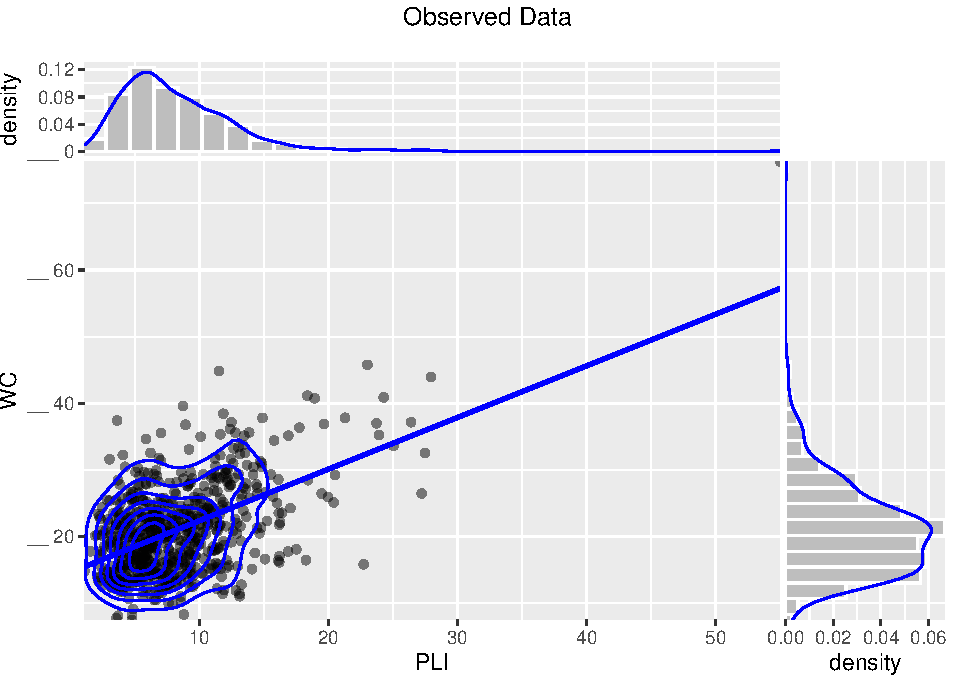
\includegraphics{figs/unnamed-chunk-6.pdf}
\caption{Observed Data}
\end{figure}

\begin{figure}
\centering
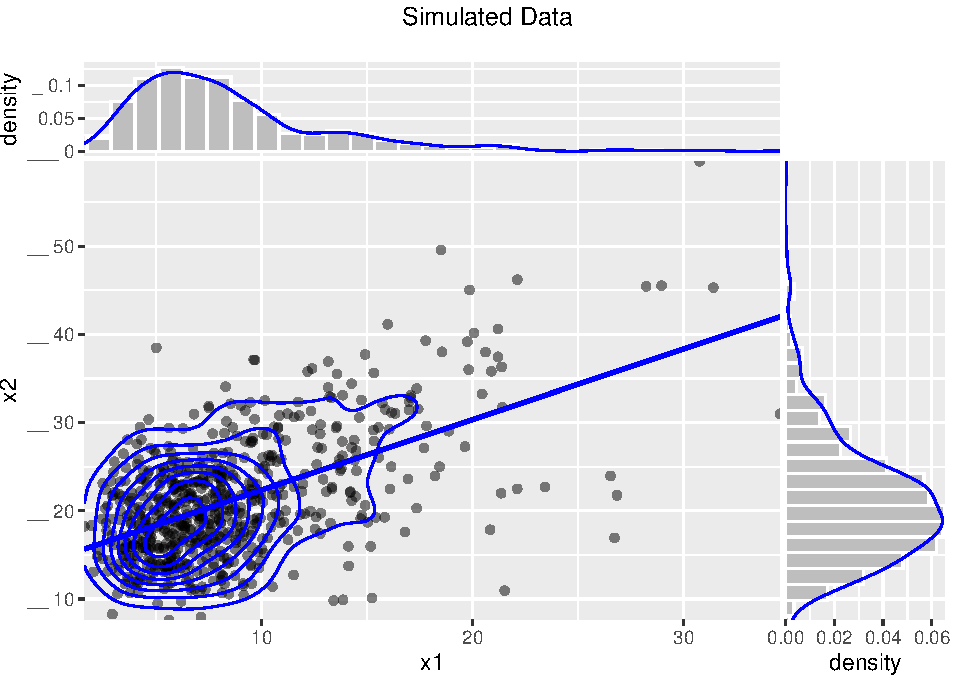
\includegraphics{figs/unnamed-chunk-7.pdf}
\caption{Simulated Data}
\end{figure}

We can see the marginal and joint distributions of observed data and
simulated data are similar, which is a good sign of our implementation.

We can also check change in data distributions when we tune the
parameters using our simulation function. Currently
\(\hat{\mu_{1}},= 1.982, \hat{\sigma_{1}}=0.513,\hat{\mu_{2}}=2.997,\hat{\sigma_{2}}=0.311,\hat{\theta}=1.608\).

First, we increase \(\theta\) to 4. The results are shown in Figure 4.
We can see with a bigger theta, the data are more correlated with
smaller deviation from the linear regression line.

\begin{figure}
\centering
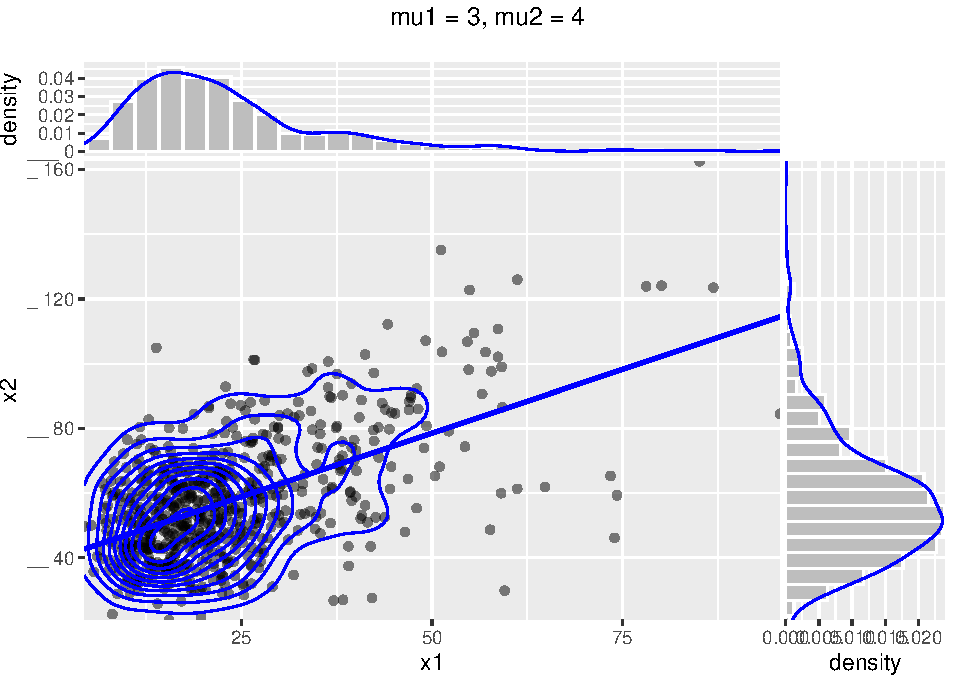
\includegraphics{figs/unnamed-chunk-8.pdf}
\caption{theta = 4}
\end{figure}

Next, we check the distribution with bigger \(\mu_1=3, \mu_2=4\). The
results are shown in Figure 5. We can see when we increase
\(\mu_1,\mu_2\), the center of the contour also shifts in the same
direction.

\begin{figure}
\centering
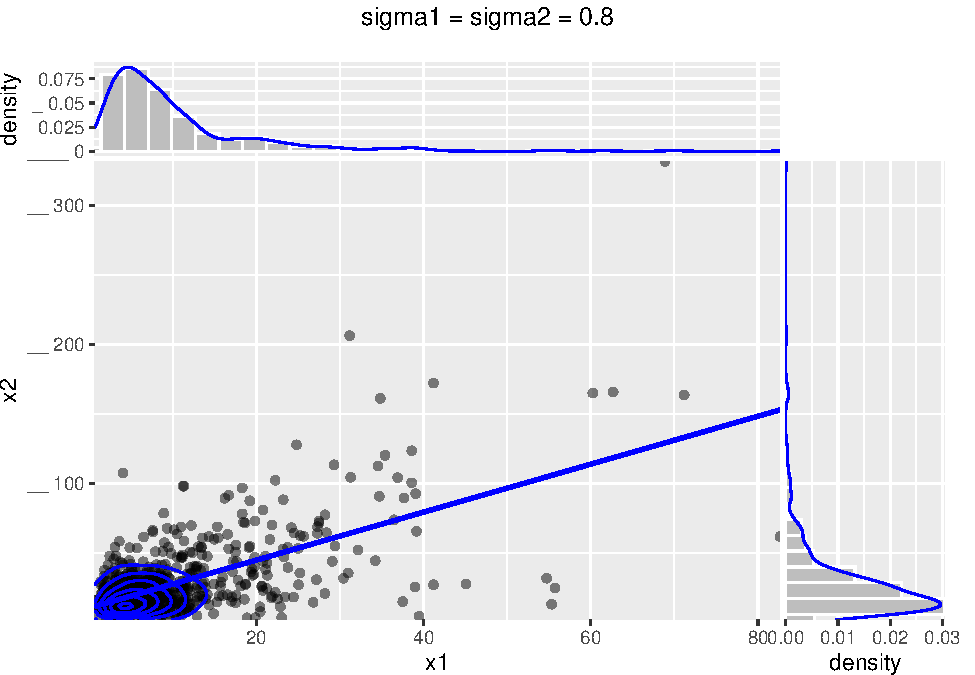
\includegraphics{figs/unnamed-chunk-9.pdf}
\caption{mu1 = 3, mu2 = 4}
\end{figure}

Next, we check the distribution with bigger standard deviation of
Lognormal distribution: \(\sigma_1 =\sigma_2 = 0.8\). The results are
shown in Figure 6. We can see that the data is more dispersed, which is
same as expected. We can also observe that a small change in
\(\sigma_1, \sigma_2\) has a big influence on the extreme values. This
is partly because the \(\sigma\) is on the log scale.

\begin{figure}
\centering
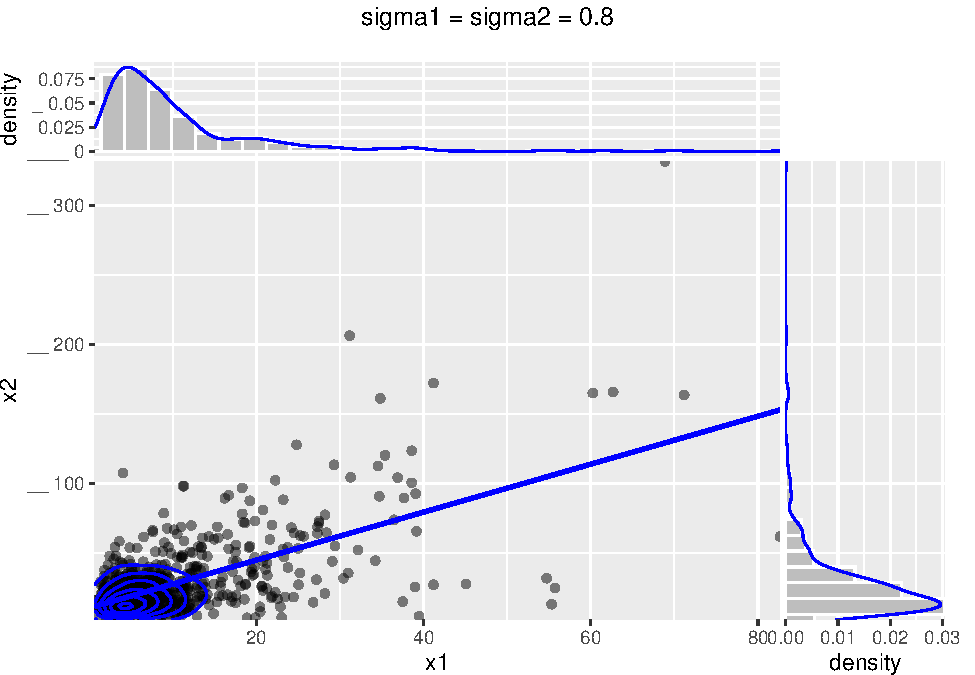
\includegraphics{figs/unnamed-chunk-10.pdf}
\caption{sigma1 = sigma2 = 0.8}
\end{figure}

\hypertarget{simulation-study}{%
\section{Simulation Study}\label{simulation-study}}

\hypertarget{acuracy-evaluation}{%
\subsection{Acuracy evaluation}\label{acuracy-evaluation}}

To evaluate how accurate our parameter estimation can be, we conduct a
simulation study assuming the following values for true parameters:
\(\mu_1=1,\sigma_1=2,\mu_2=3,\sigma_2=0.5,\theta=2\).

We compute the RMSE for 100 simulation runs of 200,500 and 1000 data
points.

\begin{figure}
\centering
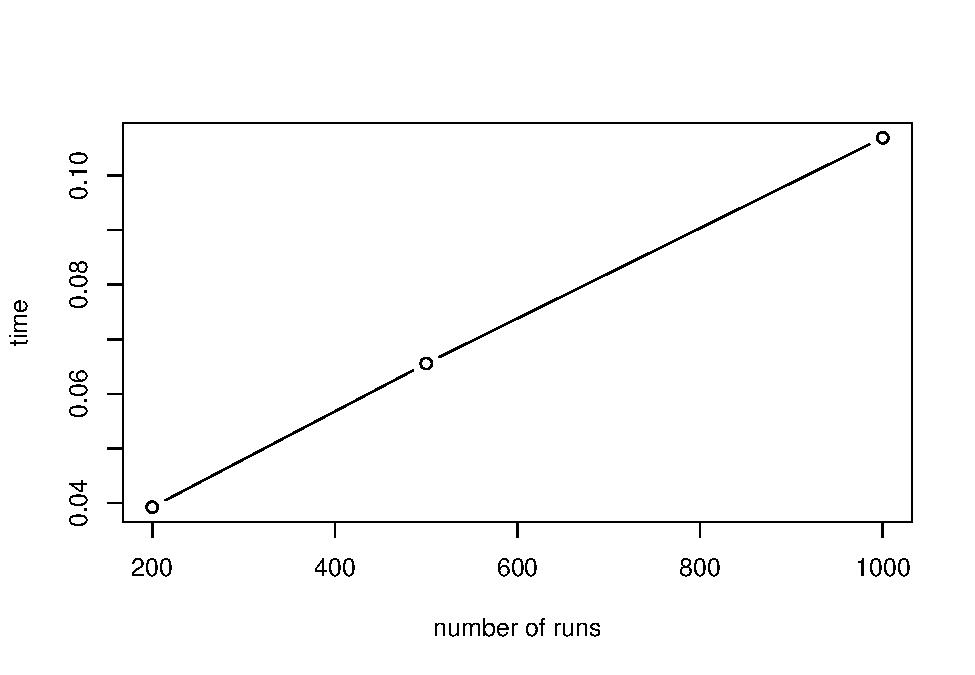
\includegraphics{figs/unnamed-chunk-14.pdf}
\caption{Average computing time vs number of runs}
\end{figure}

\begin{figure}
\centering
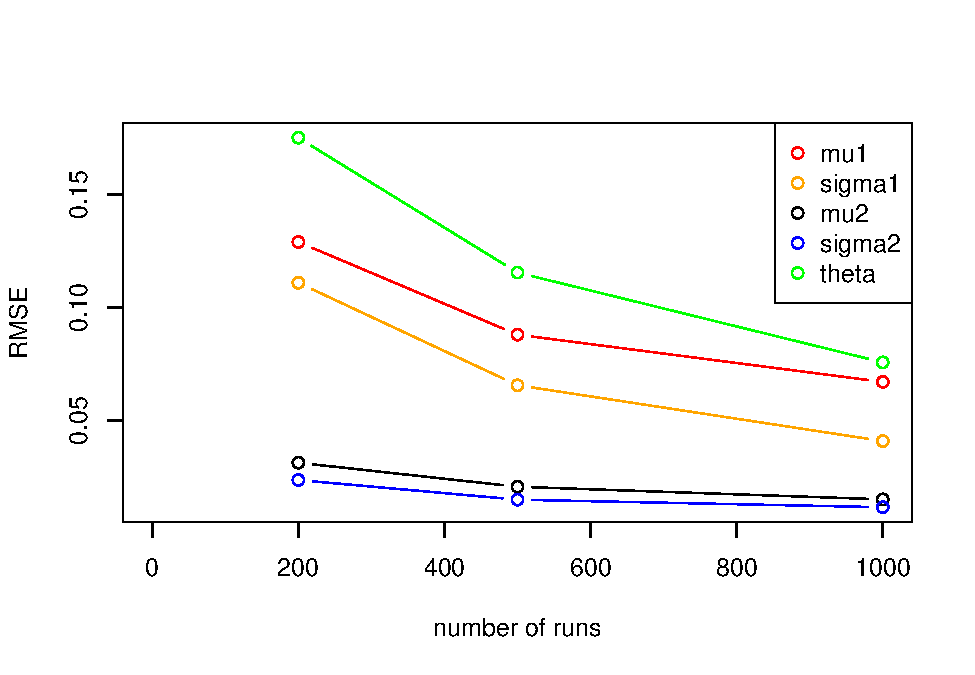
\includegraphics{figs/unnamed-chunk-15.pdf}
\caption{RMSE vs number of runs}
\end{figure}

The average computing time and RMSE are shown in Figure 7 and Figure 8.
We can see that required computation time increase linearly with the
number of runs. RMSE gets smaller with more simulation runs. \(\theta\)
is the hardest parameter to estimate with largest RMSE.
\(\mu_1, \sigma_1\) have higher RMSE than \(\mu_2, \sigma_2\)
separately. This is probably due to a lower standard deviation for
\(f_{X_2}\) (0.5 compared to 2 on the log scale). The distribution for
\(f_{X_1}\) is more dispersed, leading to a larger RMSE for
\(\mu_1, \sigma_1\).

\hypertarget{working-on-the-real-data-vt}{%
\subsection{Working on the real data:
V(t)}\label{working-on-the-real-data-vt}}

Having a feeling of the simulation models, we fit all the five
parameters to the observed data. We compute the expected payout of the
reinsurance \(V(t)\) using parametric Monte Carlo simulation (based on
the estimated parameters). We use \(10^5\) Monte Carlo samples and
calculate expected \(V(t), t=100,110,…,200\), as the average over the
simulation runs.

The plot of \(V(t)\) for \(t=100,110,…,200\) based on \(10^5\) Monte
Carlo samples is shown in Figure 9.

{[}1{]} ``P(t) and V(t) based on 10\^{}5 simulutation samples''

\begin{longtable}[]{@{}lrrrr@{}}
\toprule
& P(t) & V(t) & Std for V(t) & P(t) \textless{} V(t)\tabularnewline
\midrule
\endhead
100 & 0.0249950 & 0.0305661 & 1.8318015 & 1\tabularnewline
110 & 0.0059901 & 0.0108184 & 1.1414797 & 1\tabularnewline
120 & 0.0014355 & 0.0074188 & 0.9579313 & 1\tabularnewline
130 & 0.0003440 & 0.0000000 & 0.0000000 & 0\tabularnewline
140 & 0.0000824 & 0.0000000 & 0.0000000 & 0\tabularnewline
150 & 0.0000198 & 0.0000000 & 0.0000000 & 0\tabularnewline
160 & 0.0000047 & 0.0000000 & 0.0000000 & 0\tabularnewline
170 & 0.0000011 & 0.0000000 & 0.0000000 & 0\tabularnewline
180 & 0.0000003 & 0.0000000 & 0.0000000 & 0\tabularnewline
190 & 0.0000001 & 0.0000000 & 0.0000000 & 0\tabularnewline
200 & 0.0000000 & 0.0000000 & 0.0000000 & 0\tabularnewline
\bottomrule
\end{longtable}

\begin{figure}
\centering
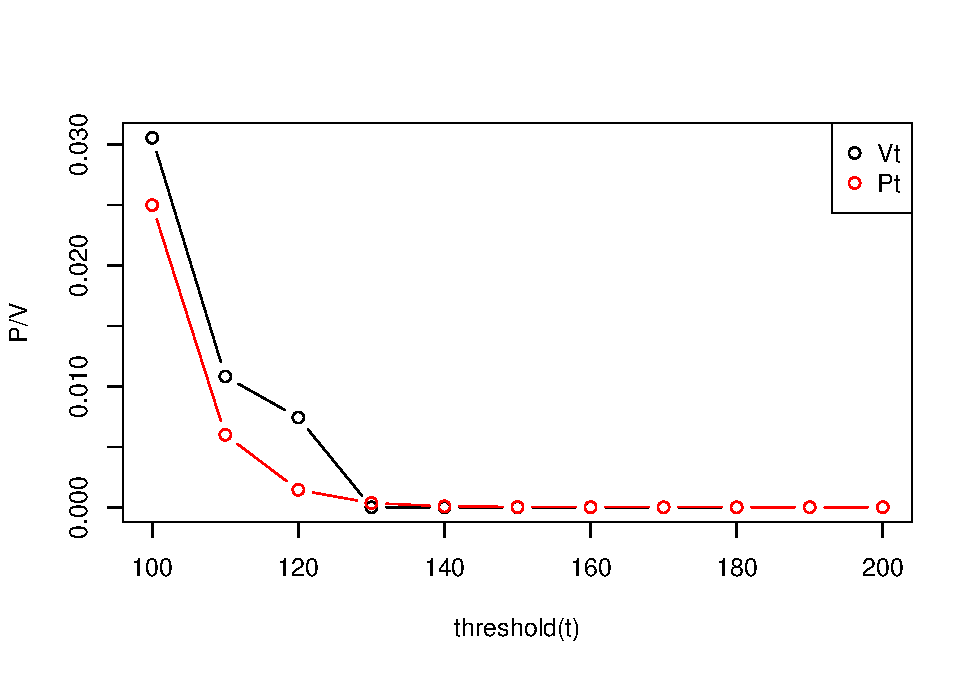
\includegraphics{figs/unnamed-chunk-20.pdf}
\caption{P(t) vs t}
\end{figure}

Based on the results, buying the reinsurance policy seems a good idea
when \(t\leq120\) since the policy price (\(P(t)\))is smaller than the
potential cost of not buying the policy (\(V(t)\)). However, the
standard deviation is high for \(V(t)\). This is because the claim
exceeding \(t\) is a highly improbable event.

\hypertarget{importance-sampling}{%
\subsection{Importance sampling}\label{importance-sampling}}

To handle the highly improbable events, we must get more samples of
claims exceeding \(t\). Therefore, importance sampling comes to play. It
is implemented by sampling from an alternative distribution that has
higher densities in the region of our interest. In our case, the
alternative density function is the Copula function with new
\(u_{1}^{\textrm{new}},u_{2}^{\textrm{new}}\).
\(u_{1}^{\textrm{new}} = \hat{u_1} + 1 ,u_{2}^{\textrm{new}}= \hat{u_2}+1\).
We adjust our estimate using an adjustment factor, which is the ratio of
the alternative distribution density and the original distribution
density.

The plot of \(V(t)\) for \(t=100,110,…,200\) based on \(10^5\) Monte
Carlo samples and importance sampling is shown in Figure 10. The
\(V(t)\) based on importance sampling have values when \(t>120\). Based
on the results, the company should buy the reinsurance policy regardless
of the value of \(t\) since \(P(t) < V(t)\).

{[}1{]} ``P(t) and V(t) based on importance sampling''

\begin{longtable}[]{@{}lrrrr@{}}
\toprule
& P(t) & V(t) & Std of V(t) & P(t) \textless{} V(t)\tabularnewline
\midrule
\endhead
100 & 0.0249950 & 0.0267185 & 0.2083507 & 1\tabularnewline
110 & 0.0059901 & 0.0117026 & 0.1244900 & 1\tabularnewline
120 & 0.0014355 & 0.0054778 & 0.0782729 & 1\tabularnewline
130 & 0.0003440 & 0.0026791 & 0.0502820 & 1\tabularnewline
140 & 0.0000824 & 0.0012372 & 0.0318883 & 1\tabularnewline
150 & 0.0000198 & 0.0005347 & 0.0187541 & 1\tabularnewline
160 & 0.0000047 & 0.0002972 & 0.0128362 & 1\tabularnewline
170 & 0.0000011 & 0.0001426 & 0.0084551 & 1\tabularnewline
180 & 0.0000003 & 0.0000781 & 0.0062483 & 1\tabularnewline
190 & 0.0000001 & 0.0000463 & 0.0047873 & 1\tabularnewline
200 & 0.0000000 & 0.0000201 & 0.0029700 & 1\tabularnewline
\bottomrule
\end{longtable}

\begin{figure}
\centering
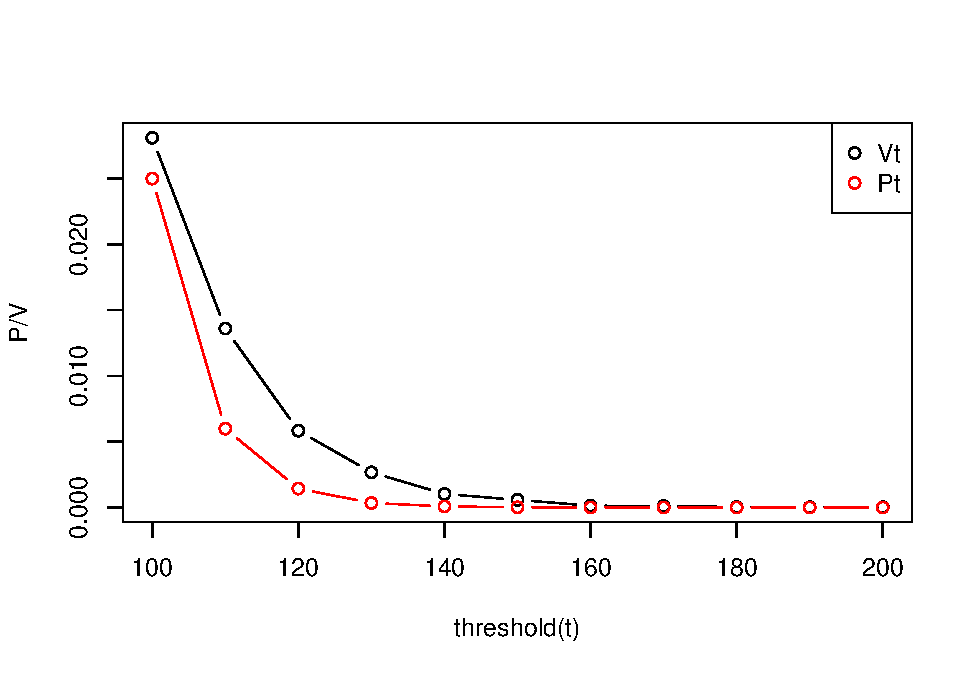
\includegraphics{figs/unnamed-chunk-25.pdf}
\caption{P(t) and V(t) vs t based on importance sampling}
\end{figure}

\hypertarget{confidence-intervals}{%
\subsection{Confidence Intervals}\label{confidence-intervals}}

Since we are not sure how confident we are about our estimates, we can
to conduct bootstrapping to get confidence intervals of \(V(t)\). The
codes doing a bootstrap method (1000 times) to compute 80\% confidence
intervals for \(V(t)\) are shown below. After getting 1000 results, we
can calculate the confidence intervals by getting the 10th and 90th
percentiles. The Confidence Intervals for \(V(t)\) are shown in Figure
11.

{[}1{]} ``P(t) and the 90\% confidence interval of V(t)''

\begin{longtable}[]{@{}lrrr@{}}
\toprule
& P(t) & Lower bound of CI(V(t)) & P(t) \textless{}
V(t)\_Lower\tabularnewline
\midrule
\endhead
100 & 0.0249950 & 0.0155202 & 0\tabularnewline
110 & 0.0059901 & 0.0064640 & 1\tabularnewline
120 & 0.0014355 & 0.0027785 & 1\tabularnewline
130 & 0.0003440 & 0.0012229 & 1\tabularnewline
140 & 0.0000824 & 0.0005514 & 1\tabularnewline
150 & 0.0000198 & 0.0002572 & 1\tabularnewline
160 & 0.0000047 & 0.0001214 & 1\tabularnewline
170 & 0.0000011 & 0.0000591 & 1\tabularnewline
180 & 0.0000003 & 0.0000291 & 1\tabularnewline
190 & 0.0000001 & 0.0000142 & 1\tabularnewline
200 & 0.0000000 & 0.0000066 & 1\tabularnewline
\bottomrule
\end{longtable}

\begin{figure}
\centering
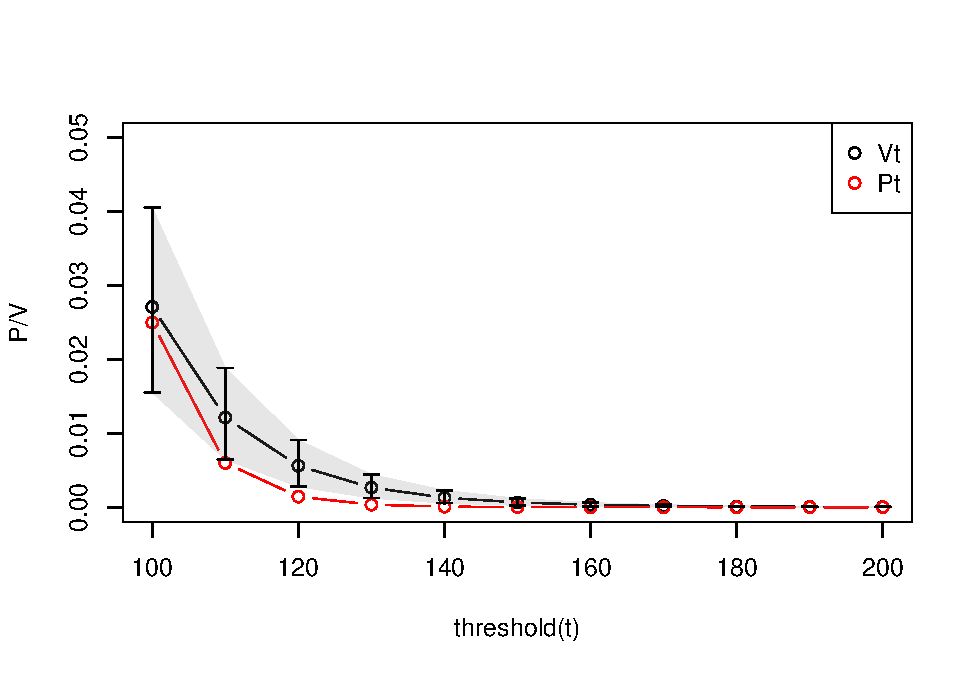
\includegraphics{figs/unnamed-chunk-31.pdf}
\caption{90\% Confidence Interval P(t) in dashed line and V(t)}
\end{figure}

\hypertarget{results}{%
\section{Results}\label{results}}

The implementation does account for Monte Carlo approximation error
since we are doing bootstrapping. However, it does not account for
estimation error since we are relying on the existing data (648 data
points).

As seen from the Figure 11, there is huge uncertainty in the values of
\(P\) when \(t\) is 100. We cannot draw a conclusion that \(V\) will be
smaller than \(P\) on a 90\% confidence level when \(t\) is 100.
However, when \(t\geq110\), the \(P\) is smaller than the lower bound of
the confidence interval \(V\), indicating that the company ANV should
buy the re-insurance.





\newpage
\singlespacing 
\bibliography{master.bib}

\end{document}
